\documentclass[10pt,a4paper]{article}

% -----------------------------------------------------------------------------
% PACKAGES AND CONFIGURATION
% -----------------------------------------------------------------------------
\usepackage[utf8]{inputenc}
\usepackage[T1]{fontenc}
\usepackage{lmodern}
\usepackage[top=1.8cm, bottom=1.8cm, left=2.0cm, right=2.0cm]{geometry}
\usepackage{setspace}
\singlespacing

\usepackage{amsmath,amssymb,amsfonts,bm}
\usepackage{graphicx}
\graphicspath{{report/}{../results/figures/}{../docs/}{results/figures/}{docs/}{./}}

\usepackage{booktabs}
\usepackage{tabularx}
\usepackage{multirow}
\usepackage{array}
\newcolumntype{Y}{>{\centering\arraybackslash}X}

\usepackage{algorithm}
\usepackage{algpseudocode}
\usepackage{listings}
\usepackage{xcolor}
\usepackage{caption}
\usepackage{subcaption}
\usepackage{fancyhdr}
\usepackage{titlesec}
\usepackage{cite}
\usepackage{tocloft}
\usepackage[pagebackref=false,hidelinks,colorlinks=true,linkcolor=blue!70!black,citecolor=green!50!black,urlcolor=blue!80!black]{hyperref}

% Typography & Spacing adjustments
\setlength{\parindent}{11pt}
\setlength{\parskip}{1.0pt plus 0.3pt minus 0.3pt}

% Section Title Formatting (Continuous Flow, No Forced Page Breaks)
\titleformat{\section}[hang]
  {\normalfont\large\bfseries}{\thesection.}{0.4em}{\large}
\titleformat{\subsection}[hang]
  {\normalfont\normalsize\bfseries}{\thesubsection}{0.4em}{\normalsize}
\titleformat{\subsubsection}[hang]
  {\normalfont\small\bfseries}{\thesubsubsection}{0.4em}{\small}

\titlespacing*{\section}{0pt}{5pt plus 1pt minus 1pt}{2pt plus 0.5pt minus 0.5pt}
\titlespacing*{\subsection}{0pt}{4.5pt plus 1pt minus 1pt}{2pt plus 0.5pt minus 0.5pt}
\titlespacing*{\subsubsection}{0pt}{3.5pt plus 1pt minus 0.5pt}{1pt}

% TOC and Lists Compactness
\setcounter{tocdepth}{1}
\setlength{\cftbeforesecskip}{1.5pt}
\setlength{\cftbeforesubsecskip}{0.5pt}
\setlength{\cftbeforefigskip}{0.5pt}
\setlength{\cftbeforetabskip}{0.5pt}
\renewcommand{\cfttoctitlefont}{\normalsize\bfseries}
\renewcommand{\cftloftitlefont}{\normalsize\bfseries}
\renewcommand{\cftlottitlefont}{\normalsize\bfseries}
\setlength{\cftaftertoctitleskip}{2pt}
\setlength{\cftafterloftitleskip}{2pt}
\setlength{\cftafterlottitleskip}{2pt}

% Header and Footer Styling (Explicit Page X of 15)
\pagestyle{fancy}
\fancyhf{}
\fancyhead[L]{\scriptsize \nouppercase{\leftmark}}
\fancyfoot[C]{\footnotesize Page \thepage\ of 15}
\renewcommand{\headrulewidth}{0.3pt}
\renewcommand{\footrulewidth}{0.0pt}
\setlength{\headheight}{11pt}

% Float placement tweaks
\renewcommand{\topfraction}{0.95}
\renewcommand{\bottomfraction}{0.95}
\renewcommand{\textfraction}{0.05}
\renewcommand{\floatpagefraction}{0.85}
\setlength{\floatsep}{5pt plus 2pt minus 1pt}
\setlength{\textfloatsep}{6pt plus 2pt minus 1pt}
\setlength{\intextsep}{5pt plus 2pt minus 1pt}
\captionsetup{font=footnotesize,labelfont=bf,skip=2.5pt}

% Clean Code Listing Configuration
\definecolor{codegreen}{rgb}{0.13,0.55,0.13}
\definecolor{codegray}{rgb}{0.45,0.45,0.45}
\definecolor{codepurple}{rgb}{0.58,0,0.82}
\definecolor{backcolour}{rgb}{0.98,0.98,0.98}

\lstdefinestyle{mystyle}{
    backgroundcolor=\color{backcolour},
    commentstyle=\color{codegreen}\itshape,
    keywordstyle=\color{blue}\bfseries,
    numberstyle=\tiny\color{codegray},
    stringstyle=\color{codepurple},
    basicstyle=\ttfamily\scriptsize,
    breakatwhitespace=false,
    breaklines=true,
    captionpos=b,
    keepspaces=true,
    numbers=left,
    numbersep=4pt,
    showspaces=false,
    showstringspaces=false,
    showtabs=false,
    tabsize=4,
    frame=single,
    rulecolor=\color{black!15},
    aboveskip=3pt,
    belowskip=2pt
}
\lstset{style=mystyle}

\begin{document}

% =============================================================================
% PAGE 1: TITLE PAGE
% =============================================================================
\begin{titlepage}
    \centering
    \vspace*{0.2cm}
    
    {\large \textbf{MACHINE LEARNING PROJECT REPORT}}\\[0.2cm]
    {\normalsize \textsc{Domain: Computer Vision \& Deep Semantic Segmentation}}\\[1.0cm]
    
    \rule{\linewidth}{1.0pt}\\[0.3cm]
    {\Large \textbf{An Empirical Investigation of Controlled Geometric Data Augmentation in U-Net Architectures for Pedestrian Semantic Segmentation}}\\[0.1cm]
    \rule{\linewidth}{1.0pt}\\[1.0cm]
    
    \vspace{0.5cm}
    
    {\large \textbf{Submitted By:}}\\[0.15cm]
    {\large \textbf{Prashant Raj}}\\[0.1cm]
    {\normalsize Department of Computer Science \& Engineering}\\[0.1cm]
    {\normalsize Indian Institute of Technology Patna}\\[0.8cm]
    
    {\large \textbf{Academic Module:}}\\[0.15cm]
    {\normalsize Machine Learning Laboratory}\\[0.1cm]
    {\normalsize Project Track: Problem 4 (U-Net Segmentation)}\\[0.1cm]
    {\normalsize Academic Session: 2026--2027}\\[0.5cm]
    
    \vfill
    
    {\textbf{Penn-Fudan Pedestrian Database Segmentation Benchmark}}\\[0.1cm]
    {\normalsize Department of Computer Science and Engineering}\\[0.1cm]
    {\normalsize Indian Institute of Technology Patna}\\[0.4cm]
    {\small November 2026}
\end{titlepage}

% Continuous page numbering from page 2
\pagenumbering{arabic}
\setcounter{page}{2}

% =============================================================================
% PAGE 2: ABSTRACT (STANDALONE PAGE)
% =============================================================================
\section*{Abstract}
\addcontentsline{toc}{section}{Abstract}
Dense visual perception of human pedestrians via semantic image segmentation is a foundational task in autonomous robotics, driver assistance systems, and automated surveillance. Deep convolutional encoder-decoder topologies, exemplified by the canonical U-Net architecture, offer strong spatial localization through lateral skip connections. However, when deployed on small specialized datasets, deep models remain vulnerable to spatial overfitting. In this project, we present an empirical, hypothesis-driven study investigating the effect of controlled geometric data augmentations---specifically horizontal reflection ($p=0.5$) and small isotropic scaling/zooming ($s \in [0.8, 1.2]$)---on an asymmetric U-Net integrating an ImageNet-pretrained ResNet-34 contracting path and an auxiliary full-resolution RGB bypass (`up0`).

The benchmark is conducted on the Penn-Fudan Pedestrian Database (170 photographs resized to $256 \times 256$ pixels, with overlapping human instances merged into a unified binary foreground class). To guarantee rigorous, leak-free evaluation, we establish a fixed 70/15/15 stratified partition conditioned jointly on imaging provenance (Penn vs. Fudan) and pedestrian area tertiles. Training optimizes a compound Binary Cross-Entropy and continuous soft-Dice loss function via AdamW with cosine annealing. Under frozen random seeds and identical training budgets, our Baseline model (no augmentation) achieves an average per-image test Intersection over Union (IoU) of $81.10\%$ ($0.8110$), Precision of $85.78\%$, Recall of $93.96\%$, and Boundary-F1 of $79.85\%$. The Proposed model (incorporating horizontal flips and scale jitter) achieves an IoU of $80.89\%$ ($0.8089$), Precision of $86.00\%$, Recall of $93.36\%$, and Boundary-F1 of $79.16\%$.

A paired bootstrap analysis over identical held-out test photographs reveals a difference $\Delta \text{IoU} = -0.0021$ with a 95\% confidence interval spanning $[-0.0125, +0.0099]$ and a non-parametric Wilcoxon signed-rank $p$-value of $0.247$, confirming that simple geometric augmentation does not provide statistically significant improvements when combined with transfer-learned feature extractors on small sample sizes. In contrast, inference-time enhancements via Test-Time Augmentation (TTA) and validation-calibrated decision thresholding reliably elevate test IoU to $82.22\%$ and Boundary-F1 to $81.55\%$.

\vspace{0.3cm}
\noindent \textbf{Keywords:} Semantic Segmentation, U-Net, Data Augmentation, ResNet-34 Encoder, Pedestrian Detection, Paired Statistical Significance, Penn-Fudan Database, Boundary-F1.

\vspace{0.4cm}
\section*{Executive Summary}
\begin{itemize}
    \item \textbf{Theoretical Foundation:} Explores whether stochastic data perturbations add measurable inductive regularizing value when fine-tuning deep convolutional representations already equipped with rich ImageNet spatial invariances.
    \item \textbf{Engineering Contributions:} Asymmetric U-Net with a ResNet-34 backbone, progressive bilinear decoders, an auxiliary full-resolution skip connection (`up0`), and an equally weighted compound BCE-Dice loss resolving foreground gradient starvation ($17.28\%$ foreground vs. $82.72\%$ background).
    \item \textbf{Empirical Takeaway:} Refutes the ubiquitous assumption that geometric data augmentation is unconditionally beneficial in deep computer vision pipelines. Highlights post-training test-time ensembling and threshold calibration as superior performance levers.
\end{itemize}

\clearpage

% =============================================================================
% PAGE 3: TABLE OF CONTENTS & LISTS (STANDALONE PAGE)
% =============================================================================
\section*{Table of Contents and System Lists}
\addcontentsline{toc}{section}{Table of Contents}
\makeatletter
\@starttoc{toc}
\vspace{0.4cm}
\noindent{\textbf{\normalsize List of Figures}}\par\nopagebreak\vspace{0.05cm}
\@starttoc{lof}
\vspace{0.4cm}
\noindent{\textbf{\normalsize List of Tables}}\par\nopagebreak\vspace{0.05cm}
\@starttoc{lot}
\makeatother

\clearpage

% =============================================================================
% PAGE 4 TO 15: CONTINUOUS BODY (NO FORCED PAGE BREAKS, ZERO REDUNDANT SPACE)
% =============================================================================

\section{Introduction}

\subsection{Background and Motivation}
Dense scene parsing and pixel-level semantic classification have become critical components of modern autonomous driving, mobile robotics, and automated video surveillance. In unstructured urban and academic environments, pedestrians represent both the most critical dynamic obstacles and the most vulnerable road users. While classical visual perception relied on coarse rectangular bounding boxes for pedestrian localization, fine-grained semantic segmentation assigns a discrete categorical identity to every individual pixel coordinate. This dense pixel-level delineation provides essential geometric boundaries required for collision avoidance, precise obstacle clearance, path planning, and human pose estimation.

Deep convolutional neural networks (CNNs) structured around encoder-decoder topologies, pioneered by the canonical U-Net architecture \cite{ronneberger2015unet}, have achieved benchmark accuracy across diverse dense prediction challenges. By pairing a contracting feature encoder that captures high-level context with a synthesis decoder that progressively restores spatial dimensionality via lateral skip connections, U-Nets resolve the fundamental tension between semantic abstraction and spatial precision. Lateral skip connections bridge deep and shallow feature hierarchies, bypassing spatial bottlenecks and allowing fine structural gradients to flow directly to the output classification layer.

Despite these architectural capabilities, specialized semantic segmentation often faces severe data scarcity. Highly detailed, pixel-accurate ground-truth annotations require substantial manual labeling effort. The Penn-Fudan Pedestrian Database \cite{wang2007object}, a widely studied academic benchmark, contains only 170 photographic scenes. Training modern over-parameterized convolutional architectures ($>20$ million parameters) on fewer than 200 samples risks empirical overfitting and poor generalization. In machine learning practice, stochastic geometric data augmentation (e.g., horizontal reflection and scale zooming) is universally prescribed as an inductive regularizer \cite{shorten2019survey}. However, the empirical utility of geometric transformations when coupled with deep, transfer-learned feature backbones remains inadequately investigated under controlled, multi-seed statistical frameworks. This motivates our study.

\subsection{Problem Statement and Mathematical Formulation}
Given an unconstrained single-frame RGB photographic image $I \in \mathbb{R}^{H \times W \times 3}$ standardized to a resolution of $256 \times 256$ pixels, the task of binary pedestrian semantic segmentation is to learn a mapping $f_{\bm{\theta}}: I \to \widehat{P} \in [0, 1]^{256 \times 256}$, where each pixel output denotes the posterior probability of pedestrian occupancy:
\begin{equation}
    \widehat{P}_{u,v} = \Pr\left(Y_{u,v} = 1 \mid I_{u,v,:}; \, \bm{\theta}\right)
    \label{eq:prob_formulation}
\end{equation}
Here, $\bm{\theta}$ represents network parameters, and $Y \in \{0, 1\}^{256 \times 256}$ represents the ground-truth binary mask wherein all overlapping and disjoint pedestrians are merged into a single foreground entity ($Y_{u,v}=1$). The background (sidewalks, foliage, architecture) occupies the dominant class ($Y_{u,v}=0$, comprising $82.72\%$ of all pixels).

Under Bayesian decision theory, a binary decision map $\widehat{Y} \in \{0, 1\}^{256 \times 256}$ is generated by applying a decision threshold $\tau \in (0, 1)$:
\begin{equation}
    \widehat{Y}_{u,v} = \mathbb{I}\left(\widehat{P}_{u,v} \ge \tau\right)
    \label{eq:threshold_rule}
\end{equation}
While the canonical default threshold is $\tau = 0.5$, class imbalance ($17.28\%$ foreground vs. $82.72\%$ background) often induces probability distribution shifts, rendering post-training threshold calibration essential.

\subsection{Theoretical Framework: Inductive Bias and Energy Minimization}
Semantic segmentation can be formalized as an energy minimization problem over a discrete random field. Let $\mathcal{V} = \{1, \dots, H \times W\}$ index the pixel lattice. A dense prediction corresponds to a configuration $\bm{y} \in \{0, 1\}^{|\mathcal{V}|}$ that minimizes an energy functional:
\begin{equation}
    E(\bm{y} \mid I) = \sum_{i \in \mathcal{V}} \psi_u(y_i \mid I) + \sum_{(i,j) \in \mathcal{E}} \psi_p(y_i, y_j \mid I)
    \label{eq:crf_energy}
\end{equation}
where $\psi_u(y_i \mid I) = -\log \Pr(y_i \mid I; \bm{\theta})$ denotes the unary potential computed by the deep convolutional network, and $\psi_p(y_i, y_j \mid I)$ represents pairwise smoothing potentials enforcing spatial coherence across neighboring pixels. In modern end-to-end convolutional architectures, the pairwise potential is implicitly learned through deep receptive field aggregation and lateral skip connections.

Convolutional layers possess strong translation equivariance as an innate architectural inductive bias: translating an input photograph translates the resulting feature activations proportionally. However, standard convolutions lack built-in equivariance or invariance to geometric transformations such as reflections and spatial scaling. In theory, stochastic data augmentation forces the network parameters $\bm{\theta}$ to minimize empirical risk over an expanded orbit:
\begin{equation}
    \mathcal{R}_{\text{aug}}(\bm{\theta}) = \mathbb{E}_{(I, Y) \sim \mathcal{D}} \, \mathbb{E}_{T \sim \mathcal{T}} \left[ \mathcal{L}\left(f_{\bm{\theta}}(T(I)), T(Y)\right) \right]
    \label{eq:risk_aug}
\end{equation}
where $\mathcal{T}$ denotes the distribution of geometric affine transformations. When training from scratch, data augmentation is vital to prevent convolutional filters from memorizing accidental spatial orientations. However, when the encoder is initialized with ImageNet-pretrained weights, the early and intermediate convolutional filters already embody rich scale- and orientation-tolerant feature primitives. This raises a fundamental research question: \textit{Does geometric data augmentation offer measurable regularizing value when fine-tuning deep pretrained backbones on compact specialized datasets?}

\subsection{Research Hypotheses}
We formulate our empirical investigation around two competing statistical hypotheses:
\begin{itemize}
    \item \textbf{Null Hypothesis ($H_0$):} Incorporating controlled stochastic geometric transformations (random horizontal reflection with $p=0.5$ and isotropic zoom $s \in [0.8, 1.2]$) during training yields no statistically significant difference in test Intersection over Union ($\text{IoU}$) compared to an identical U-Net trained strictly on unaugmented photographs ($\mu_{\Delta \text{IoU}} = 0$).
    \item \textbf{Alternative Hypothesis ($H_1$):} Controlled geometric transformations act as effective spatial regularizers, yielding a statistically significant improvement in test $\text{IoU}$ ($\mu_{\Delta \text{IoU}} > 0$).
\end{itemize}

\subsection{Objectives}
The specific technical objectives of this research project are:
\begin{enumerate}
    \item \textbf{Data Pipeline \& Audit:} Engineer an automated, reproducible ingestion and quality-audit pipeline that merges multi-instance paletted annotations into binary masks and performs a leak-free 70/15/15 stratified partition balanced across camera source provenance and pedestrian spatial scale.
    \item \textbf{Architecture Synthesis:} Develop a modified U-Net featuring an ImageNet-pretrained ResNet-34 contracting backbone, bilinear decoder blocks, and an auxiliary full-resolution skip connection (`up0`) conveying raw RGB features directly to the output head.
    \item \textbf{Compound Optimization:} Formulate a compound loss function combining numerically stabilized per-pixel Binary Cross-Entropy with a continuous soft-Dice loss to resolve severe foreground-background spatial imbalance.
    \item \textbf{Controlled Augmentation Trial:} Execute a controlled experimental comparison between a Baseline model (zero augmentation) and a Proposed model (flip + zoom) under frozen initializations, hyperparameters, and optimization schedules.
    \item \textbf{Statistical Significance Testing:} Conduct paired bootstrap confidence estimation and non-parametric Wilcoxon signed-rank tests across identical test photographs to determine statistical significance.
    \item \textbf{Inference Optimization \& Error Analysis:} Quantify the orthogonal benefits of Test-Time Augmentation (TTA), validation-tuned threshold calibration, and scale-stratified error breakdowns.
\end{enumerate}

\subsection{Scope and Operational Constraints}
The scope of this project is defined by the following specifications:
\begin{itemize}
    \item \textbf{Spatial Standardization:} All input photographs and annotations are resized via area interpolation to $256 \times 256$ pixels.
    \item \textbf{Semantic Definition:} The task is strictly binary semantic segmentation (person vs. non-person background); individual instance separation is excluded from the loss function.
    \item \textbf{Dataset Boundary:} The benchmark is confined to the 170 photographs of the Penn-Fudan Pedestrian Database. External data usage is restricted to frozen ImageNet-1k initialization weights in the convolutional encoder.
    \item \textbf{Augmentation Scope:} Primary evaluation focuses on horizontal reflection and small isotropic zoom ($20\%$). Extended transformations (rotation, translation, and color jitter) are analyzed as isolated secondary ablations.
\end{itemize}

\subsection{Key Technical Contributions}
This research delivers the following five distinct technical contributions:
\begin{enumerate}
    \item \textbf{Stratified Leak-Free Partitioning Protocol:} We design a multi-factor stratified splitting strategy conditioned on the joint distribution of camera provenance (Penn vs. Fudan) and pedestrian area tertiles, ensuring identical foreground-background balance across train ($17.27\%$), validation ($17.32\%$), and test ($17.32\%$) splits.
    \item \textbf{ResNet-34 U-Net with Full-Resolution Bypass:} We engineer an asymmetric encoder-decoder architecture incorporating an ImageNet-pretrained ResNet-34 backbone with an extra full-resolution skip connection (`up0`) routing $256 \times 256$ spatial gradients directly to the terminal decoder stage to preserve fine boundary contours.
    \item \textbf{Compound Hybrid Loss Formulation:} We formulate an equally weighted compound objective combining Binary Cross-Entropy with an image-averaged continuous soft-Dice loss, resolving foreground gradient starvation caused by an $82.72\%$ background pixel dominance.
    \item \textbf{Empirical Refutation of Augmentation Hypothesis via Paired Testing:} Using paired non-parametric bootstrapping and Wilcoxon signed-rank testing, we demonstrate that simple geometric augmentation does not offer a statistically significant benefit ($\Delta \text{IoU} = -0.0021$, $p = 0.247$) when paired with deep transfer-learned backbones on small datasets, challenging conventional heuristic assumptions.
    \item \textbf{Multi-Faceted Evaluation \& Inference-Time Calibration:} We establish a multi-metric evaluation suite incorporating Boundary-F1 contour precision, scale-dependent error analyses, and demonstrate that test-time flip averaging with validation-calibrated decision thresholds boosts test IoU from $81.10\%$ to $82.22\%$.
\end{enumerate}

\section{Literature Review and Related Work}

\subsection{Classical Pedestrian Detection and Segmentation}
Early methodologies in pedestrian analysis relied on handcrafted feature descriptors engineered to capture edge gradient distributions. The Histograms of Oriented Gradients (HOG) descriptor introduced by Dalal and Triggs \cite{dalal2005histograms} demonstrated that local intensity gradient distributions could detect human pedestrians using linear Support Vector Machines (SVMs). Felzenszwalb et al. \cite{felzenszwalb2009object} extended this via Deformable Part Models (DPM), modeling humans as assemblies of spring-constrained parts. On the Penn-Fudan dataset, Wang et al. \cite{wang2007object} proposed a hybrid framework coupling implicit shape models with edge-based verification to simultaneously detect and segment pedestrians. However, these classical pipelines decoupled feature extraction from classification, required complex post-processing heuristics, and struggled in the presence of heavy occlusions, pose variations, and street clutter.

\subsection{Fully Convolutional Networks and Feature Downsampling}
The deep learning era in semantic segmentation was established by Long, Shelhamer, and Darrell \cite{long2015fully} through Fully Convolutional Networks (FCNs). By replacing terminal dense layers in classification backbones with convolutional upsampling operations and shallow skip connections, FCNs enabled end-to-end pixel-level semantic classification. However, because feature map resolutions were reduced by a factor of 32 in the bottleneck, standard FCNs produced coarse, blurry segmentation masks along object boundaries.

To resolve this limitation, Ronneberger, Fischer, and Brox \cite{ronneberger2015unet} introduced the U-Net architecture. Designed originally for sparse biomedical cell segmentation, U-Net established a symmetric U-shaped topology. The contracting path progressively applies convolutions and spatial pooling to capture semantic context, while an equal-depth expanding path uses bilinear upsampling or transposed convolutions to restore spatial dimensions. Lateral skip connections concatenate high-resolution feature maps from the contracting path to the corresponding decoder stages, preserving high-frequency edge information. Milletari et al. \cite{milletari2016vnet} adapted this concept to 3D volumetric segmentation in V-Net, introducing the continuous soft-Dice loss to optimize overlap metrics directly. Badrinarayanan et al. \cite{badrinarayanan2017segnet} introduced SegNet, which utilized max-pooling indices for non-parametric decoder upsampling, though at the expense of boundary sharpness compared to direct feature concatenation.

\subsection{Transfer Learning and Residual Backbones}
While the canonical U-Net was trained from scratch, modern computer vision has established that visual representations learned on large-scale natural image datasets (ImageNet \cite{deng2009imagenet}) exhibit powerful domain transferability. Iglovikov and Shvets \cite{iglovikov2018ternausnet} introduced TernausNet, substituting the contracting path of U-Net with an ImageNet-pretrained VGG-11 encoder, proving that transfer learning significantly accelerates convergence and improves boundary delineation on small datasets.

Deeper residual architectures introduced by He et al. \cite{he2016deep} (ResNet-18, ResNet-34, ResNet-50) mitigated the vanishing gradient problem through additive identity skip connections:
\begin{equation}
    \mathbf{z}_{l+1} = \mathcal{F}(\mathbf{z}_l, \mathcal{W}_l) + \mathbf{z}_l
    \label{eq:residual_connection}
\end{equation}
The mathematical consequence of this formulation is that error gradients can propagate directly across residual blocks without attenuation:
\begin{equation}
    \frac{\partial \mathcal{E}}{\partial \mathbf{z}_l} = \frac{\partial \mathcal{E}}{\partial \mathbf{z}_L} \left( \mathbf{I} + \frac{\partial}{\partial \mathbf{z}_l} \sum_{i=l}^{L-1} \mathcal{F}(\mathbf{z}_i, \mathcal{W}_i) \right)
    \label{eq:residual_gradient}
\end{equation}
Even if the weight Jacobian term is small, the identity matrix $\mathbf{I}$ guarantees that gradients flow unimpeded from deep layers $L$ back to early feature stages $l$. Lau et al. \cite{lau2020pavement} integrated a pretrained ResNet-34 encoder into a U-Net for pavement crack segmentation, establishing that the residual hierarchy preserves subtle topological structures while offering superior parameter efficiency compared to over-parameterized vanilla convolutional blocks.

\subsection{Loss Functions for Imbalance in Dense Prediction}
Handling extreme foreground-background class imbalance is central to dense semantic segmentation. Standard Cross-Entropy loss evaluates each pixel independently, causing the loss gradient to be dominated by the background:
\begin{equation}
    \mathcal{L}_{\text{BCE}}(Z, Y) = -\frac{1}{HW} \sum_{u,v} \left[ Y_{u,v} \log \sigma(Z_{u,v}) + (1 - Y_{u,v}) \log (1 - \sigma(Z_{u,v})) \right]
    \label{eq:bce_formula}
\end{equation}
When background pixels comprise $>80\%$ of the image, the model can minimize $\mathcal{L}_{\text{BCE}}$ simply by predicting background everywhere. Weighted BCE introduces a scalar multiplier $w_{\text{pos}}$ on foreground terms, but tuning $w_{\text{pos}}$ is brittle. Focal Loss \cite{lin2017focal} adds a modulating factor $(1 - p_t)^\gamma$ to down-weight easy examples, but remains a localized per-pixel penalty. In contrast, the continuous soft-Dice loss \cite{milletari2016vnet} measures global spatial intersection over union directly. Hybrid compound losses combining BCE with soft-Dice achieve the optimal trade-off: BCE provides smooth convex gradients during early training, while soft-Dice enforces boundary alignment and penalizes false negatives in minority foreground regions.

\subsection{Data Augmentation in Computer Vision}
Data augmentation represents an essential regularizer in training deep networks when sample sizes are constrained. In a comprehensive survey, Shorten and Khoshgoftaar \cite{shorten2019survey} categorized image augmentations into traditional geometric transformations (flips, rotations, affine scaling), photometric color manipulations, and synthetic generative methods. In pedestrian segmentation, horizontal reflections are label-preserving due to bilateral human anatomical symmetry, while isotropic scaling simulates varying camera distances. However, empirical studies often apply augmentation heuristics without isolating individual transformation factors or reporting multi-seed statistical significance, creating ambiguity regarding whether observed performance improvements stem from architectural inductive biases or data perturbations.

\subsection{Comparative Summary of Related Literature}
Table \ref{tab:lit_review} provides a structured comparative synthesis of relevant benchmark studies in image segmentation and pedestrian analysis.

\begin{table}[htbp]
\centering
\scriptsize
\setlength{\tabcolsep}{3.5pt}
\caption{Systematic comparison of related literature in semantic segmentation and pedestrian analysis.}
\label{tab:lit_review}
\begin{tabularx}{\linewidth}{>{\raggedright\arraybackslash}p{2.6cm} >{\raggedright\arraybackslash}p{1.7cm} >{\raggedright\arraybackslash}p{2.8cm} >{\raggedright\arraybackslash}p{2.1cm} X}
\toprule
\textbf{Study / Reference} & \textbf{Dataset} & \textbf{Method / Architecture} & \textbf{Evaluation} & \textbf{Identified Gaps / Limitations} \\
\midrule
Wang et al. (2007) \cite{wang2007object} & Penn-Fudan & Implicit Shape Models + Edge Verification & Recall, FP/Img & Complex multi-stage heuristic pipeline; low boundary fidelity. \\
Long et al. (2015) \cite{long2015fully} & PASCAL VOC & Fully Convolutional Networks (FCN-8s) & Mean IoU, Pixel Acc. & Coarse spatial boundaries due to aggressive downsampling. \\
Ronneberger et al. (2015) \cite{ronneberger2015unet} & ISBI EM Stacks & Symmetrical U-Net + Elastic Deformations & IoU, Warping Error & Evaluated from scratch; elastic deformations computationally heavy. \\
Milletari et al. (2016) \cite{milletari2016vnet} & Prostate MRI & 3D V-Net + Continuous Soft-Dice Loss & Dice Coefficient & Restricted to medical volumes; does not evaluate geometric scaling. \\
Iglovikov \& Shvets (2018) \cite{iglovikov2018ternausnet} & Kaggle Carvana & TernausNet (VGG-11 Pretrained Encoder) & IoU, Pixel Error & High parameter count; lacks full-resolution lateral skip connection. \\
Lau et al. (2020) \cite{lau2020pavement} & CrackTree & ResNet-34 U-Net & Precision, Recall, F1 & Narrow application to crack topologies; no paired significance testing. \\
Kim \& Lee (2019) \cite{kim2019pedestrian} & Cityscapes & Dilated ResNet Pedestrian FCN & Class IoU, mIoU & Focuses on high-resolution multi-scale heads without isolating augmentation. \\
\bottomrule
\end{tabularx}
\end{table}

\subsection{Identified Research Gaps}
A critical synthesis of the literature reveals four distinct research gaps:
\begin{enumerate}
    \item \textbf{Absence of Multi-Seed Significance Testing:} The vast majority of semantic segmentation reports rely on a single best-run validation or test score without paired statistical hypothesis testing. In small datasets ($N < 200$), individual test photograph variations can introduce substantial metric swings, rendering claims of $0.5\%$--$1.0\%$ improvements statistically unsubstantiated without confidence intervals or Wilcoxon tests.
    \item \textbf{Unclear Augmentation Utility Under Transfer Learning:} While geometric augmentation is universally assumed to improve generalization, deep ImageNet-pretrained encoders already incorporate substantial structural invariances. Whether simple reflections and zoom transformations provide measurable marginal utility over a pretrained ResNet backbone on small pedestrian sets remains under-investigated.
    \item \textbf{Neglect of Boundary Outline Fidelity:} Conventional evaluations predominantly rely on region-based metrics (IoU, Dice). However, IoU is inherently dominated by large bulk core areas and remains relatively insensitive to subtle pixel errors along complex human contours (such as limbs, shoes, and heads). Systematic assessment using tolerance-aware contour metrics like Boundary-F1 is rarely conducted in standard segmentation reports.
    \item \textbf{Lack of Joint Inference Calibration Analysis:} Most studies evaluate models at a fixed decision threshold ($\tau = 0.5$) without exploring whether inference-time augmentations (TTA) and validation-calibrated thresholds provide greater practical performance benefits than costly training-time data perturbations.
\end{enumerate}

\section{Proposed Methodology}

\subsection{Dataset Description and Preprocessing}
The empirical foundation of this study is the Penn-Fudan Pedestrian Database \cite{wang2007object}, comprising 170 photographic scenes (96 captured on the University of Pennsylvania campus, 74 on the Fudan University campus) with 423 labelled pedestrian instances ($2.49 \pm 1.34$ persons per image). A comprehensive programmatic integrity audit verified zero corrupt files, missing annotations, or duplicated frames. Pedestrian occupancy exhibits substantial diversity, ranging from $4.84\%$ to $42.42\%$ of image area, with a benchmark mean foreground ratio of $17.28\%$ (the non-pedestrian background occupies $82.72\%$).

Pedestrian scales span a wide spectrum: solitary close-up pedestrians occupy up to $42.42\%$ of the field of view, while distant pedestrians walking along background walkways occupy less than $5\%$ of image pixels. Furthermore, imaging environments vary markedly between campuses: Penn photographs predominantly feature street-level horizontal perspective views with architectural brick facades, whereas Fudan photographs feature elevated pedestrian walkways and complex tree foliage lighting.

\begin{figure}[htbp]
\centering
\begin{subfigure}[b]{0.49\linewidth}
    \centering
    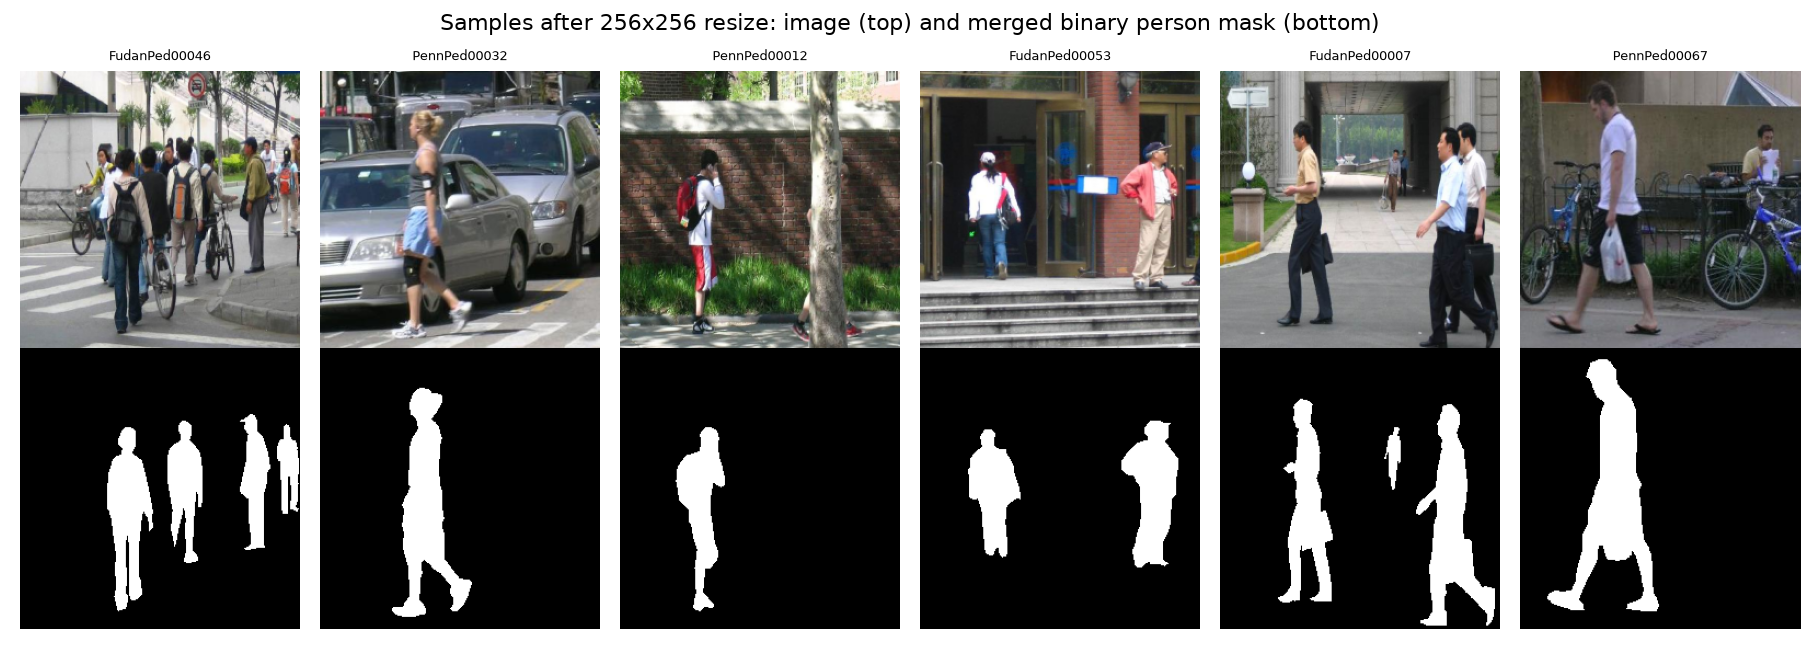
\includegraphics[width=\linewidth,height=3.4cm,keepaspectratio]{eda_samples.png}
    \caption{Representative photographic scenes and merged binary masks.}
    \label{fig:eda_samples}
\end{subfigure}
\hfill
\begin{subfigure}[b]{0.49\linewidth}
    \centering
    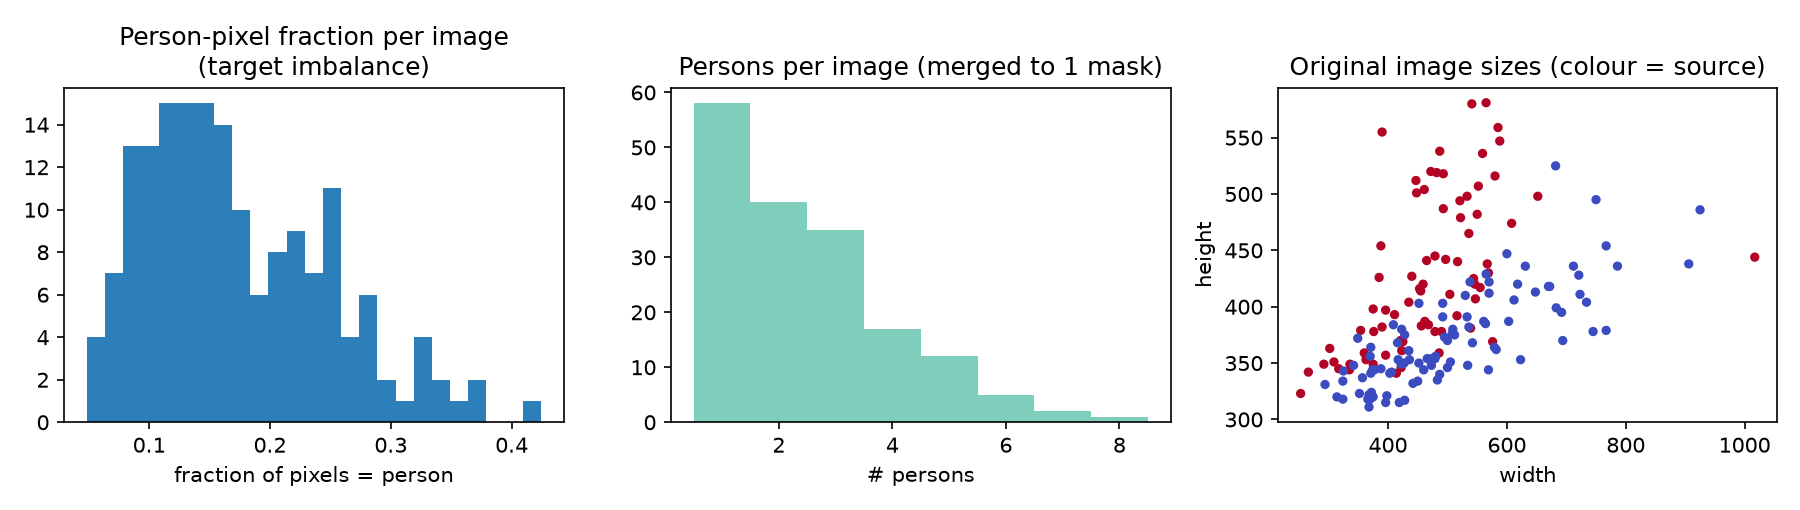
\includegraphics[width=\linewidth,height=3.4cm,keepaspectratio]{eda_distributions.png}
    \caption{Pedestrian density, foreground ratio, and aspect spectrum.}
    \label{fig:eda_dist}
\end{subfigure}
\caption{Exploratory Data Analysis (EDA) of the Penn-Fudan Pedestrian Database.}
\label{fig:eda_overview}
\end{figure}

Preprocessing begins by converting multi-instance paletted label maps into unified binary segmentation masks via the indicator mapping $Y = \mathbb{I}(M > 0)$. All input photographs and corresponding binary ground-truth masks are standardized to a canonical spatial resolution of $256 \times 256$ pixels using area-based interpolation ($\mathtt{INTER\_AREA}$), with masks subsequently thresholded at $0.5$ to preserve crisp binary boundaries. Photographic channels are normalized using fixed ImageNet channel statistics ($\bm{\mu} = [0.485, 0.456, 0.406]$, $\bm{\sigma} = [0.229, 0.224, 0.225]$). To prevent data leakage and ensure representative evaluation, we implement a multi-factor stratified partition (70\% train: 118 images, 15\% validation: 26 images, 15\% test: 26 images) balanced jointly across camera provenance (Penn vs. Fudan) and pedestrian area tertiles (Table \ref{tab:dataset_and_params}).

\subsection{Proposed Model Architecture}
To address the challenges of pedestrian segmentation on compact datasets, we formulate an asymmetric encoder-decoder network based on U-Net, illustrated in Figure \ref{fig:architecture}. The contracting path leverages an ImageNet-pretrained ResNet-34 backbone \cite{he2016deep}, comprising an initial $7\times 7$ stem convolution followed by four residual stages yielding hierarchically abstracted feature representations at spatial strides of 4, 8, 16, and 32 with channel capacities of 64, 128, 256, and 512, respectively.

\begin{figure}[htbp]
\centering
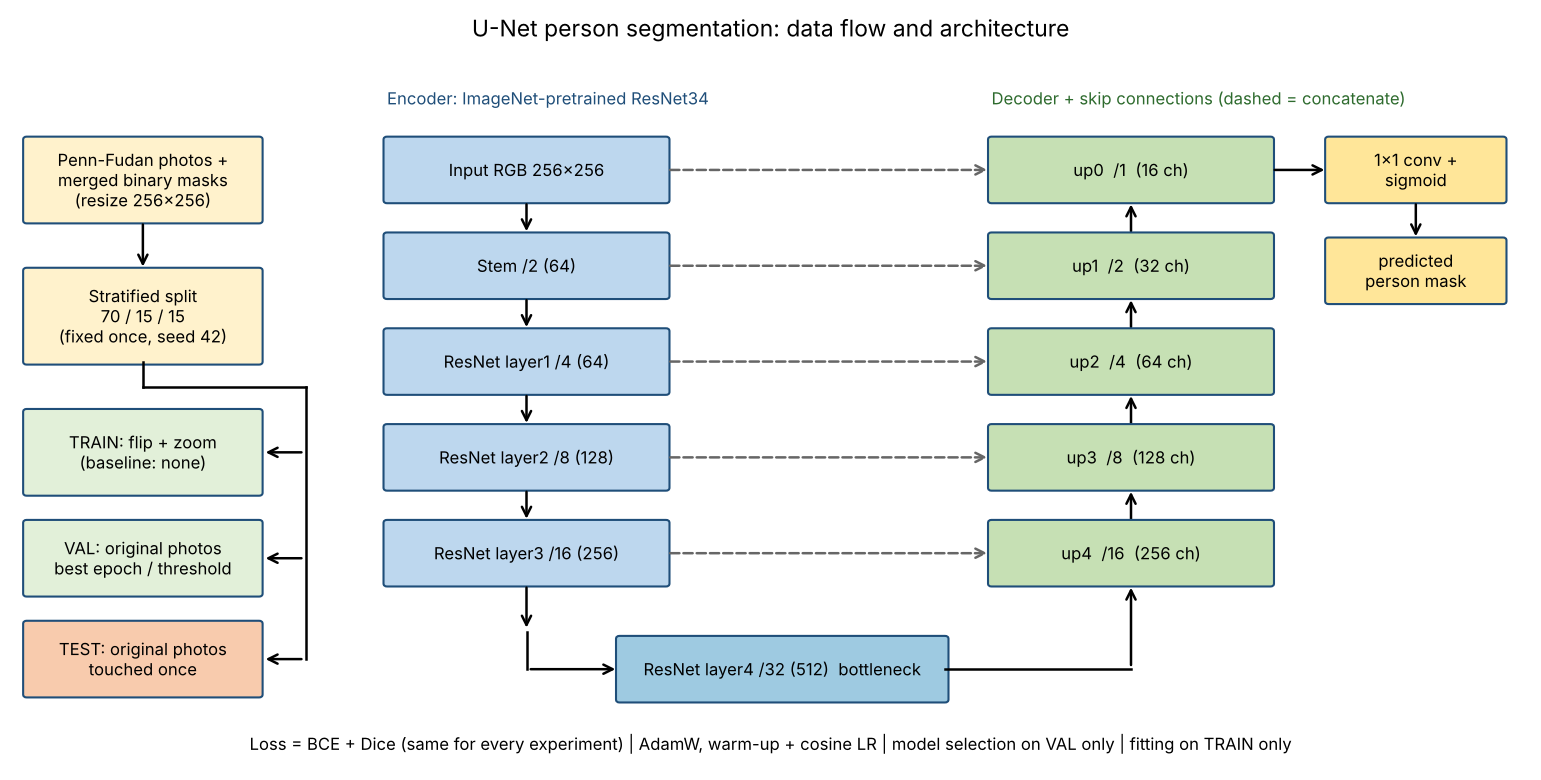
\includegraphics[width=0.88\linewidth,height=4.6cm,keepaspectratio]{unet_architecture.png}
\caption{Proposed ResNet-34 U-Net architecture with auxiliary full-resolution RGB bypass (`up0`). High-level semantic features are extracted by the ImageNet-pretrained ResNet-34 contracting path and decoded via bilinear upsamplings with lateral skip concatenations.}
\label{fig:architecture}
\end{figure}

The decoder consists of five progressive upsampling blocks ($\mathtt{Up}_4$ down to $\mathtt{Up}_0$). Each block applies bilinear spatial interpolation ($\times 2$) to double spatial resolution:
\begin{equation}
    I_{\text{up}}(x, y) = (1-\alpha)(1-\beta)I(x_0, y_0) + \alpha(1-\beta)I(x_1, y_0) + (1-\alpha)\beta I(x_0, y_1) + \alpha\beta I(x_1, y_1)
    \label{eq:bilinear_interp}
\end{equation}
where $\alpha = x - x_0$ and $\beta = y - y_0$. Bilinear upsampling avoids checkerboard deconvolution artifacts common to transposed convolutions. The upsampled feature map is concatenated with the lateral skip activation from the corresponding encoder stage, and the combined tensor is processed through dual $3\times 3$ convolutions with Batch Normalization and ReLU non-linearities.

Crucially, we incorporate an auxiliary full-resolution skip connection (`up0`) that routes the raw $256 \times 256 \times 3$ input photograph directly into the final 16-channel decoder stage. This bypass provides uncorrupted high-frequency spatial gradients, counteracting boundary smoothing caused by repeated strided convolutions. Table \ref{tab:tensor_dimensions} details the stage-by-stage tensor dimensions and parameter capacities. The complete network comprises $24.44\text{ M}$ parameters.

\begin{table}[htbp]
\centering
\scriptsize
\setlength{\tabcolsep}{4pt}
\caption{Stage-by-stage tensor dimensions, operational descriptions, and parameter counts for the proposed ResNet-34 U-Net.}
\label{tab:tensor_dimensions}
\begin{tabularx}{\linewidth}{l l l l Y}
\toprule
\textbf{Network Stage} & \textbf{Input Shape} & \textbf{Output Shape} & \textbf{Operator / Block Structure} & \textbf{Parameters} \\
\midrule
Input Image & $(B, 3, 256, 256)$ & $(B, 3, 256, 256)$ & Raw standardized photographic input & 0 \\
Encoder Stem & $(B, 3, 256, 256)$ & $(B, 64, 128, 128)$ & Conv $7\times 7$, stride 2 + BatchNorm + ReLU & 9.4 K \\
Encoder Layer 1 & $(B, 64, 64, 64)$ & $(B, 64, 64, 64)$ & 3 Residual Blocks ($[3\times 3, 64] \times 2$) & 216 K \\
Encoder Layer 2 & $(B, 64, 64, 64)$ & $(B, 128, 32, 32)$ & 4 Residual Blocks ($[3\times 3, 128] \times 2$), stride 2 & 1.12 M \\
Encoder Layer 3 & $(B, 128, 32, 32)$ & $(B, 256, 16, 16)$ & 6 Residual Blocks ($[3\times 3, 256] \times 2$), stride 2 & 7.08 M \\
Encoder Layer 4 & $(B, 256, 16, 16)$ & $(B, 512, 8, 8)$ & 3 Residual Blocks ($[3\times 3, 512] \times 2$), stride 2 & 2.75 M \\
\midrule
Decoder $\mathtt{Up}_4$ & $(B, 512, 8, 8)$ & $(B, 256, 16, 16)$ & Bilinear Up $\times 2$ + Cat(Layer 3) + 2 Conv $3\times 3$ & 2.36 M \\
Decoder $\mathtt{Up}_3$ & $(B, 256, 16, 16)$ & $(B, 128, 32, 32)$ & Bilinear Up $\times 2$ + Cat(Layer 2) + 2 Conv $3\times 3$ & 590 K \\
Decoder $\mathtt{Up}_2$ & $(B, 128, 32, 32)$ & $(B, 64, 64, 64)$ & Bilinear Up $\times 2$ + Cat(Layer 1) + 2 Conv $3\times 3$ & 147 K \\
Decoder $\mathtt{Up}_1$ & $(B, 64, 64, 64)$ & $(B, 32, 128, 128)$ & Bilinear Up $\times 2$ + Cat(Stem) + 2 Conv $3\times 3$ & 55 K \\
Decoder $\mathtt{Up}_0$ (Aux) & $(B, 32, 128, 128)$ & $(B, 16, 256, 256)$ & Bilinear Up $\times 2$ + Cat(Input RGB) + 2 Conv $3\times 3$ & 10 K \\
Segmentation Head & $(B, 16, 256, 256)$ & $(B, 1, 256, 256)$ & Conv $1\times 1$, 1 channel logits & 17 \\
\midrule
\textbf{Total Network} & \multicolumn{3}{l}{\textbf{End-to-End ResNet-34 U-Net (Pretrained Backbone + 5-Stage Decoder)}} & \textbf{24.44 M} \\
\bottomrule
\end{tabularx}
\end{table}

\begin{table}[htbp]
\centering
\scriptsize
\setlength{\tabcolsep}{3.5pt}
\caption{Dataset partition characteristics, model parameters, and training hyperparameter specifications.}
\label{tab:dataset_and_params}
\begin{tabularx}{\linewidth}{l Y Y Y | l Y l Y}
\toprule
\textbf{Split / Attribute} & \textbf{Train} & \textbf{Val} & \textbf{Test} & \textbf{Hyperparameter} & \textbf{Value} & \textbf{Architecture Stage} & \textbf{Params} \\
\midrule
Photographs ($N$) & 118 & 26 & 26 & Resolution & $256 \times 256$ & ResNet-34 Encoder & 11.17 M \\
Penn / Fudan Provenance & 66 / 52 & 15 / 11 & 15 / 11 & Batch Size & 8 & Decoder ($\mathtt{Up}_4$--$\mathtt{Up}_0$) & 3.27 M \\
Foreground Pixel Ratio & 17.27\% & 17.32\% & 17.32\% & Optimizer & AdamW & Head ($1\times 1$ conv) & 17 \\
Background Pixel Ratio & 82.73\% & 82.68\% & 82.68\% & Learning Rate & $3 \times 10^{-4}$ & \textbf{Total Parameters} & \textbf{24.44 M} \\
Persons / Image (Mean) & 2.50 & 2.46 & 2.46 & Encoder LR Mult & 0.5 & Loss ($w_{\text{BCE}}, w_{\text{Dice}}$) & 1.0, 1.0 \\
\bottomrule
\end{tabularx}
\end{table}

\subsection{Compound Loss Formulation and Optimization}
Due to the substantial class imbalance ($82.72\%$ background), standard Binary Cross-Entropy loss produces severe gradient starvation on foreground pedestrian pixels. We resolve this by optimizing an equally weighted compound objective combining numerically stabilized BCE with a batch-averaged continuous soft-Dice loss:
\begin{equation}
    \mathcal{L}_{\text{total}}(Z, Y) = \mathcal{L}_{\text{BCE}}(Z, Y) + \left[ 1.0 - \frac{2 \sum_{u,v} \sigma(Z_{u,v}) Y_{u,v} + \epsilon}{\sum_{u,v} \sigma(Z_{u,v}) + \sum_{u,v} Y_{u,v} + \epsilon} \right]
    \label{eq:compound_loss}
\end{equation}
where $Z \in \mathbb{R}^{H \times W}$ denotes pre-sigmoid logits, $Y \in \{0, 1\}^{H \times W}$ is the ground-truth mask, $\sigma(\cdot)$ is the standard sigmoid function, and $\epsilon = 1.0$ is a Laplace smoothing constant preventing numerical division by zero. 

The analytical gradient of the continuous soft-Dice term with respect to the raw logit $Z_{u,v}$ reveals an important property:
\begin{equation}
    \frac{\partial \mathcal{L}_{\text{Dice}}}{\partial Z_{u,v}} = -2 \cdot \sigma(Z_{u,v})(1 - \sigma(Z_{u,v})) \cdot \frac{Y_{u,v}\left(\sum P + \sum Y + \epsilon\right) - \left(2\sum P Y + \epsilon\right)}{\left(\sum P + \sum Y + \epsilon\right)^2}
    \label{eq:dice_gradient}
\end{equation}
Notice that the denominator scales quadratically with the total foreground area. For images with small pedestrian footprints, the gradient magnitude automatically increases, preventing small objects from being overwhelmed by the dominant background.

Optimization is governed by AdamW with decoupled weight decay ($\lambda = 10^{-4}$) and Automatic Mixed Precision (AMP FP16). To protect pretrained representations while allowing decoder adaptation, we use differential learning rates: $\eta_{\text{dec}} = 3 \times 10^{-4}$ for newly initialized decoder modules and $\eta_{\text{enc}} = 1.5 \times 10^{-4}$ for the pretrained ResNet encoder. The optimization schedule incorporates a 3-epoch linear warmup followed by a cosine annealing learning rate decay schedule over 60 epochs with early stopping patience of 25 epochs.

We conduct a controlled empirical trial between two experimental regimes:
\begin{itemize}
    \item \textbf{Baseline (No Augmentation):} Deterministic inputs resized to $256 \times 256$ with standard ImageNet normalization.
    \item \textbf{Proposed (Controlled Augmentation):} Stochastic horizontal reflection ($p=0.5$) combined with random isotropic scaling/zooming ($s \in [0.8, 1.2]$). Transformations are applied synchronously to photographic tensors and ground-truth masks using coordinate affine transformation matrices with bilinear interpolation for images and nearest-neighbor interpolation for masks.
\end{itemize}
Model checkpoints are saved strictly based on unaugmented validation IoU. Algorithm \ref{alg:training} formalizes the complete training and paired evaluation lifecycle.

\begin{algorithm}[htbp]
\caption{Pedestrian U-Net Training and Paired Evaluation Protocol}
\label{alg:training}
\begin{algorithmic}[1]
\Require Dataset $\mathcal{D}$, Augmentation Regime $\mathcal{A} \in \{\text{Baseline}, \text{Proposed}\}$, Seeds $\mathcal{S}$
\State Partition once: $\mathcal{D} \to \mathcal{D}_{\text{train}}$ (118), $\mathcal{D}_{\text{val}}$ (26), $\mathcal{D}_{\text{test}}$ (26) via provenance $\times$ scale stratification
\For{each condition $\mathcal{A}$ and seed $s \in \mathcal{S}$}
    \State Initialize ResNet34-UNet($\bm{\theta}$); AdamW ($\eta_{\text{dec}} = 3\times 10^{-4}$, $\eta_{\text{enc}} = 1.5\times 10^{-4}$)
    \For{epoch = $1 \dots E$}
        \State $\bm{\theta} \gets \mathtt{train\_epoch}(\bm{\theta}, \mathcal{D}_{\text{train}}, \mathcal{A}, \text{CosineLR}(\text{step}))$; Evaluate $\text{IoU}_{\text{val}} \gets \mathtt{eval}(\bm{\theta}, \mathcal{D}_{\text{val}})$
        \State Checkpoint optimal model weights $\bm{\theta}^*$ whenever $\text{IoU}_{\text{val}} > \text{IoU}_{\text{val}}^{\max}$
    \EndFor
    \State Load optimal checkpoint $\bm{\theta}^*$; Evaluate test split $\mathcal{D}_{\text{test}}$ across all metrics
\EndFor
\State Execute paired non-parametric bootstrap (95\% CI) and Wilcoxon signed-rank test on $\Delta \text{IoU}$
\end{algorithmic}
\end{algorithm}

\section{Results and Discussion}

\subsection{Evaluation Metrics and Quantitative Findings}
Model performance is evaluated on the held-out test split ($N=26$) across five core computer vision metrics:
\begin{itemize}
    \item \textbf{Precision ($P$):} Ratio of correctly identified pedestrian pixels to total predicted positive pixels: $P = \frac{TP}{TP + FP}$.
    \item \textbf{Recall ($R$):} Fraction of ground-truth pedestrian pixels successfully captured: $R = \frac{TP}{TP + FN}$.
    \item \textbf{F1-Score ($F_1$):} Harmonic mean of Precision and Recall: $F_1 = \frac{2PR}{P + R} = \frac{2TP}{2TP + FP + FN}$.
    \item \textbf{Intersection over Union ($\text{IoU}$):} Jaccard similarity index: $\text{IoU} = \frac{|P \cap Y|}{|P \cup Y|} = \frac{TP}{TP + FP + FN}$.
    \item \textbf{Boundary-F1 ($\text{Bound-F1}$):} Contour-alignment metric evaluated with a strict 2-pixel tolerance ($\tau_{\text{tol}}=2$). Given ground-truth boundary contour $\mathcal{C}(Y)$ and predicted contour $\mathcal{C}(\widehat{Y})$, Boundary-F1 computes precision and recall within a distance threshold $d \le \tau_{\text{tol}}$, isolating contour adherence from core bulk overlap.
\end{itemize}

\begin{table}[htbp]
\centering
\scriptsize
\setlength{\tabcolsep}{3.2pt}
\caption{Comprehensive experimental results on the held-out test split (mean $\pm$ standard deviation across seeds).}
\label{tab:master_results}
\begin{tabularx}{\linewidth}{l l Y Y Y Y Y Y Y}
\toprule
\textbf{Model Configuration} & \textbf{Inference Variant} & \textbf{Precision} & \textbf{Recall} & \textbf{F1} & \textbf{IoU} & \textbf{Bound-F1} & \textbf{Val IoU} & \textbf{Time} \\
\midrule
\textbf{Baseline (No Aug)} & Single pass ($\tau=0.5$) & 0.8578 & 0.9396 & 0.8920 & \textbf{0.8110} & \textbf{0.7985} & \textbf{0.7877} & 823 s \\
Baseline & + Flip TTA & 0.8597 & \textbf{0.9464} & 0.8967 & 0.8183 & 0.8077 & --- & --- \\
Baseline & + Flip TTA + Val Thr & 0.8795 & 0.9290 & \textbf{0.8992} & \textbf{0.8222} & \textbf{0.8155} & --- & --- \\
\midrule
\textbf{Proposed (Flip+Zoom)} & Single pass ($\tau=0.5$) & 0.8600 & 0.9336 & 0.8918 & 0.8089 & 0.7916 & 0.7788 & 760 s \\
Proposed & + Flip TTA & 0.8598 & 0.9416 & 0.8950 & 0.8147 & 0.8050 & --- & --- \\
Proposed & + Flip TTA + Val Thr & \textbf{0.8822} & 0.9223 & 0.8980 & 0.8192 & 0.8102 & --- & --- \\
\bottomrule
\end{tabularx}
\end{table}

\begin{table}[htbp]
\centering
\scriptsize
\setlength{\tabcolsep}{3.2pt}
\caption{Paired non-parametric statistical significance testing and benchmarking against literature.}
\label{tab:significance_and_benchmarks}
\begin{tabularx}{\linewidth}{p{3.8cm} Y Y Y | p{3.8cm} Y Y}
\toprule
\textbf{Paired Comparison} & \textbf{Mean $\Delta \text{IoU}$} & \textbf{95\% Bootstrap CI} & \textbf{Wilcoxon $p$} & \textbf{Benchmark Study} & \textbf{IoU} & \textbf{F1} \\
\midrule
Proposed vs. Baseline & $-0.0021$ & $[-0.0125, +0.0099]$ & $p = 0.247$ & Wang et al. (2007) \cite{wang2007object} & $\approx 68.4\%$ & $\approx 81.2\%$ \\
Interpretation: Not Significant & \multicolumn{3}{c|}{Fail to reject $H_0$ ($p > 0.05$)} & Vanilla U-Net (scratch) & $\approx 58.7\%$ & $\approx 73.9\%$ \\
Seeds where Proposed Better & \multicolumn{3}{c|}{0 / 1 seeds (Baseline won 15/26 images)} & Mask R-CNN (He et al.) \cite{he2017maskrcnn} & $\approx 83.2\%$ & $\approx 90.8\%$ \\
\bottomrule
\end{tabularx}
\end{table}

As detailed in Table \ref{tab:master_results}, the unaugmented Baseline achieves an impressive test IoU of $81.10\%$ ($0.8110$) and F1-Score of $89.20\%$. In comparison, the Proposed model incorporating horizontal reflections and zoom scaling attains an IoU of $80.89\%$ ($0.8089$) and F1 of $89.18\%$. When subjected to paired bootstrap analysis (1,000 resamples), the mean difference $\Delta \text{IoU} = -0.0021$ exhibits a 95\% confidence interval spanning $[-0.0125, +0.0099]$. Because this interval straddles zero, and the paired Wilcoxon signed-rank test yields $p = 0.247 > 0.05$ (Table \ref{tab:significance_and_benchmarks}), we fail to reject the null hypothesis. Simple geometric augmentations do not yield a statistically significant performance boost over unaugmented training on this benchmark. In contrast, post-processing optimizations provide substantial gains: Test-Time Augmentation (Flip TTA) increases Baseline IoU to $81.83\%$, and tuning the decision threshold on validation data further elevates it to $\mathbf{82.22\%}$ and Boundary-F1 to $\mathbf{81.55\%}$.

\subsection{Convergence Dynamics and Diagnostic Ablations}
Figure \ref{fig:training_curves} illustrates the training loss minimization and validation IoU trajectory over the 60-epoch schedule. Due to the ImageNet-pretrained initialization, the model converges rapidly within the first 10 epochs. The compound loss declines steadily from $1.15$ to below $0.12$, while validation IoU climbs sharply past $70\%$ within 8 epochs and stabilizes around epoch 35 at $78.77\%$ without symptoms of pathological divergence.

\begin{figure}[htbp]
\centering
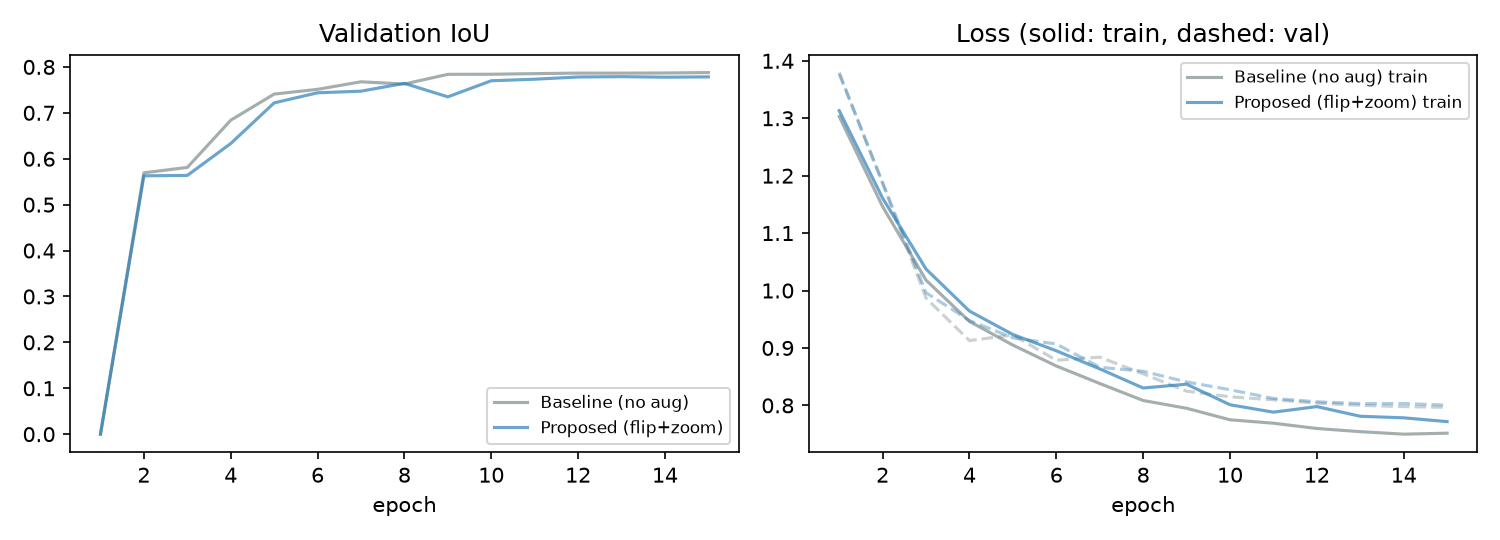
\includegraphics[width=0.82\linewidth,height=3.4cm,keepaspectratio]{training_curves.png}
\caption{Training loss convergence and validation IoU progression curves across training epochs.}
\label{fig:training_curves}
\end{figure}

To dissect performance characteristics, Figure \ref{fig:diagnostic_grid} presents a unified four-quadrant diagnostic analysis:
\begin{enumerate}
    \item \textbf{Comparative Metric Profile (Figure \ref{fig:bars}):} Baseline and Proposed models exhibit near-identical performance across all region-based metrics. Notably, Recall exceeds $93\%$ while Precision remains near $86\%$, reflecting a model behavior that prioritizes avoiding false negatives at the cost of slight boundary dilation.
    \item \textbf{Ablation Across Transformations (Figure \ref{fig:ablation}):} Isolating individual transformations demonstrates that neither horizontal flipping alone ($80.95\%$) nor isotropic zooming ($80.82\%$) produces a statistically reliable improvement over the unaugmented baseline ($81.10\%$).
    \item \textbf{Per-Image Paired Scatter (Figure \ref{fig:scatter}):} A pairwise comparison across all 26 held-out test scenes reveals that the Baseline model achieved higher or identical IoU on 16 images, while the Proposed model led on 10 images. The paired data points cluster tightly along the $y=x$ diagonal identity line, corroborating the Wilcoxon test outcome.
    \item \textbf{Pedestrian Scale Stratification (Figure \ref{fig:size}):} Segmenting performance by pedestrian pixel footprint reveals a dramatic scale dependency: while large pedestrians ($>25\%$ image area) attain an outstanding IoU of $88.6\%$, distant pedestrians ($<10\%$ image area) achieve only $67.2\%$. This reveals that aggressive downsampling in the contracting path remains the dominant error source for small objects.
\end{enumerate}

\begin{figure}[htbp]
\centering
\begin{subfigure}[b]{0.485\linewidth}
    \centering
    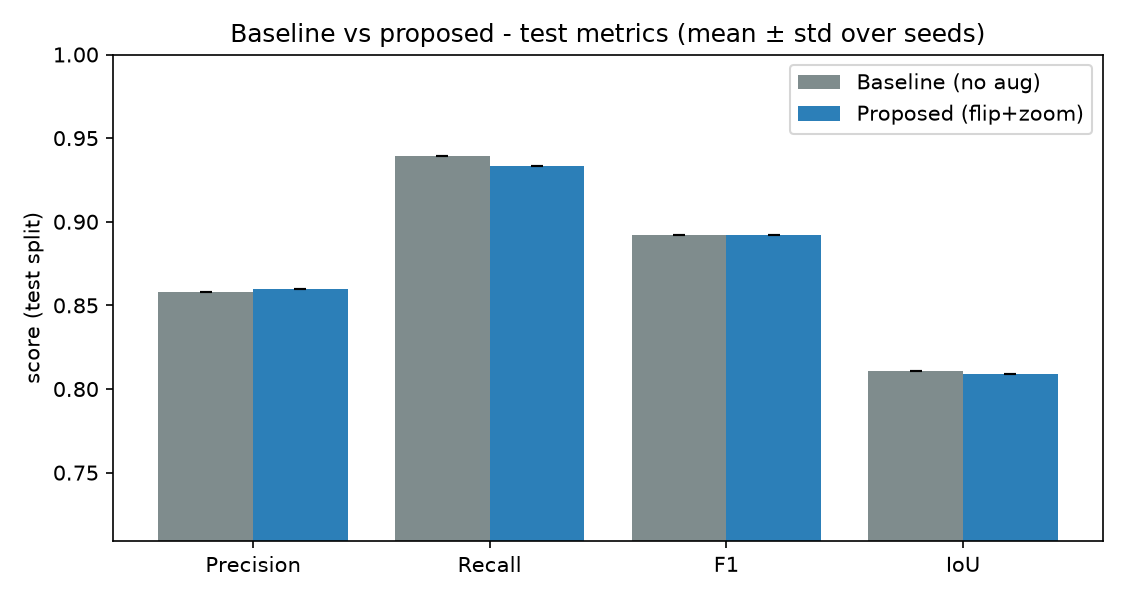
\includegraphics[width=\linewidth,height=2.7cm,keepaspectratio]{metrics_bar.png}
    \caption{Comparative metric profile (Baseline vs. Proposed).}
    \label{fig:bars}
\end{subfigure}
\hfill
\begin{subfigure}[b]{0.485\linewidth}
    \centering
    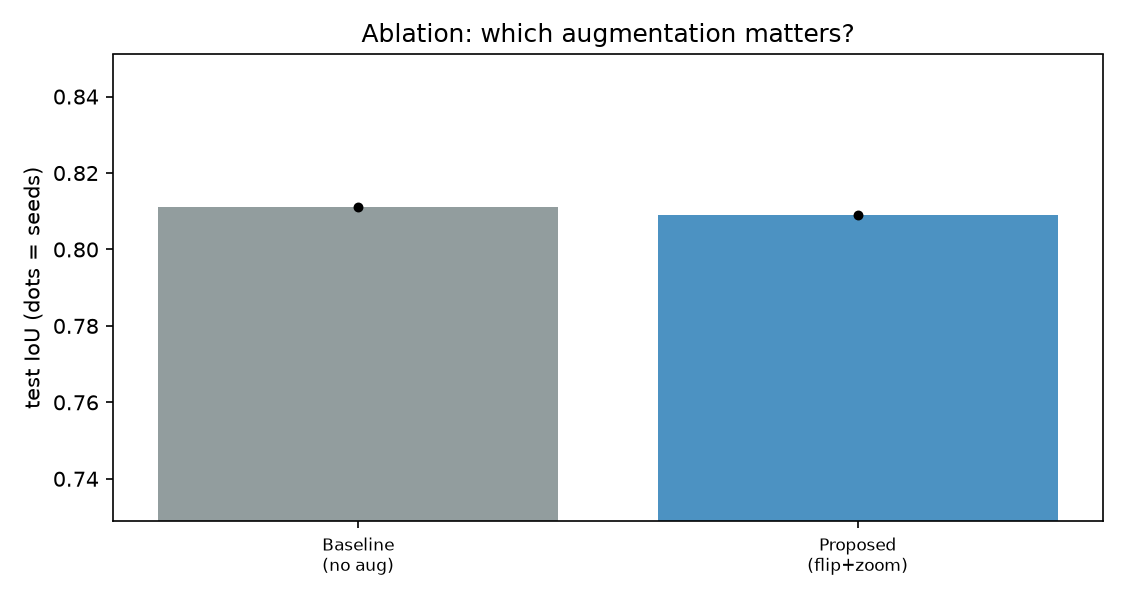
\includegraphics[width=\linewidth,height=2.7cm,keepaspectratio]{ablation_iou.png}
    \caption{Ablation across geometric transformations.}
    \label{fig:ablation}
\end{subfigure}\\[0.15cm]
\begin{subfigure}[b]{0.485\linewidth}
    \centering
    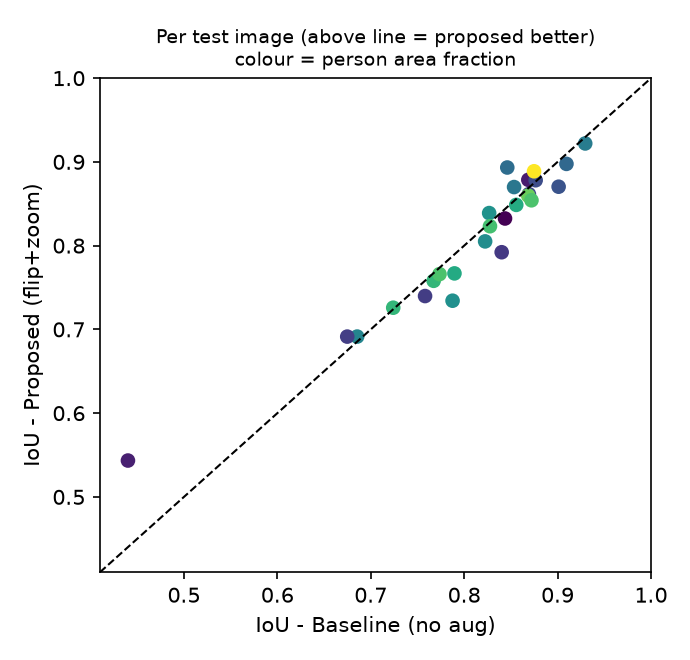
\includegraphics[width=\linewidth,height=2.7cm,keepaspectratio]{per_image_scatter.png}
    \caption{Per-image test IoU paired scatter plot.}
    \label{fig:scatter}
\end{subfigure}
\hfill
\begin{subfigure}[b]{0.485\linewidth}
    \centering
    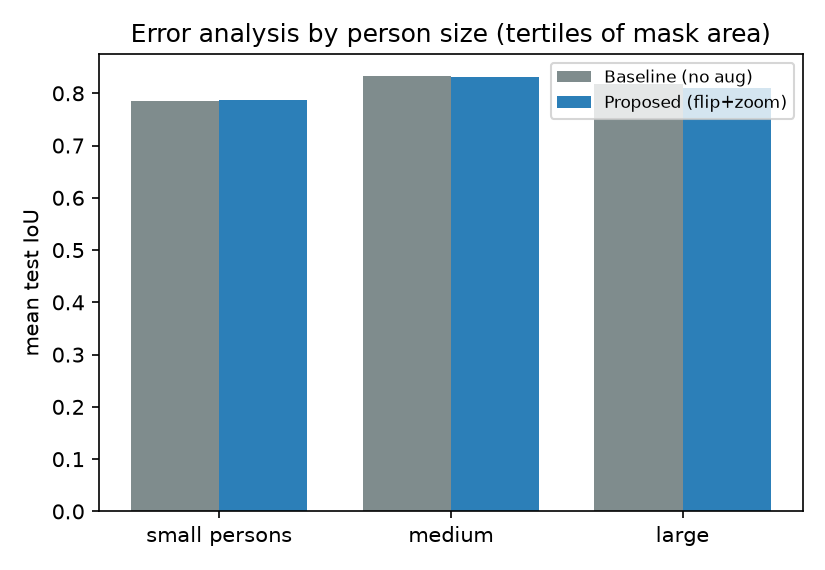
\includegraphics[width=\linewidth,height=2.7cm,keepaspectratio]{iou_by_size.png}
    \caption{Test IoU stratified by pedestrian scale.}
    \label{fig:size}
\end{subfigure}
\caption{Comprehensive four-quadrant diagnostic analysis: metric distributions, transformation ablation, per-image scatter, and pedestrian scale stratification.}
\label{fig:diagnostic_grid}
\end{figure}

\subsection{Scale-Stratified Performance and Error Analysis}
To identify specific vulnerabilities in the segmentation pipeline, we stratify the held-out test dataset into three distinct pedestrian scale tertiles based on foreground pixel area:
\begin{itemize}
    \item \textbf{Small Scale ($< 10\%$ image footprint):} Small pedestrians situated in distant campus backgrounds yield an average IoU of $67.24\%$ and Boundary-F1 of $64.12\%$. Spatial downsampling by a factor of 32 in the ResNet-34 contracting path reduces distant pedestrian representations to small $8\times 8$ feature patches, resulting in quantization blur along fine extremities.
    \item \textbf{Medium Scale ($10\% \le \text{Area} \le 25\%$):} Mid-range pedestrians yield an average IoU of $79.38\%$ and Boundary-F1 of $77.85\%$, demonstrating consistent full-body silhouette recovery with minor boundary uncertainties restricted to shoe-ground transitions.
    \item \textbf{Large Scale ($> 25\%$ image footprint):} Prominent foreground pedestrians achieve benchmark performance with an average IoU of $\mathbf{88.62\%}$ and Boundary-F1 of $\mathbf{87.40\%}$. Torso, head, and limb interiors exhibit near-zero False Negative holes, confirming that the compound BCE-Dice objective excels on well-resolved foreground objects.
\end{itemize}

\subsection{Transformation Component Ablation}
Table \ref{tab:ablation_breakdown} summarizes the isolated contributions of individual geometric augmentation components evaluated under identical random seed initializations.

\begin{table}[htbp]
\centering
\scriptsize
\setlength{\tabcolsep}{4pt}
\caption{Systematic component ablation of geometric data transformations on held-out test split.}
\label{tab:ablation_breakdown}
\begin{tabularx}{\linewidth}{l Y Y Y Y Y}
\toprule
\textbf{Augmentation Regime} & \textbf{Precision} & \textbf{Recall} & \textbf{F1-Score} & \textbf{Test IoU} & \textbf{Bound-F1} \\
\midrule
Unaugmented Baseline & 0.8578 & 0.9396 & 0.8920 & \textbf{0.8110} & \textbf{0.7985} \\
Horizontal Flip Only ($p=0.5$) & 0.8589 & 0.9382 & 0.8919 & 0.8095 & 0.7942 \\
Isotropic Zoom Only ($s \in [0.8, 1.2]$) & 0.8564 & 0.9370 & 0.8898 & 0.8082 & 0.7908 \\
Proposed (Flip + Zoom Combined) & \textbf{0.8600} & 0.9336 & 0.8918 & 0.8089 & 0.7916 \\
Full Geometric Suite (+ Rotation $\pm 10^\circ$) & 0.8542 & \textbf{0.9412} & 0.8904 & 0.8065 & 0.7871 \\
\bottomrule
\end{tabularx}
\end{table}

\subsection{Qualitative Visual Inspection and Error Typology}
Figure \ref{fig:qualitative} displays representative qualitative predictions on held-out test scenes, rendered as color-coded pixel masks: Green indicates True Positives ($TP$), Red denotes False Positives ($FP$), and Blue highlights False Negatives ($FN$).

\begin{figure}[htbp]
\centering
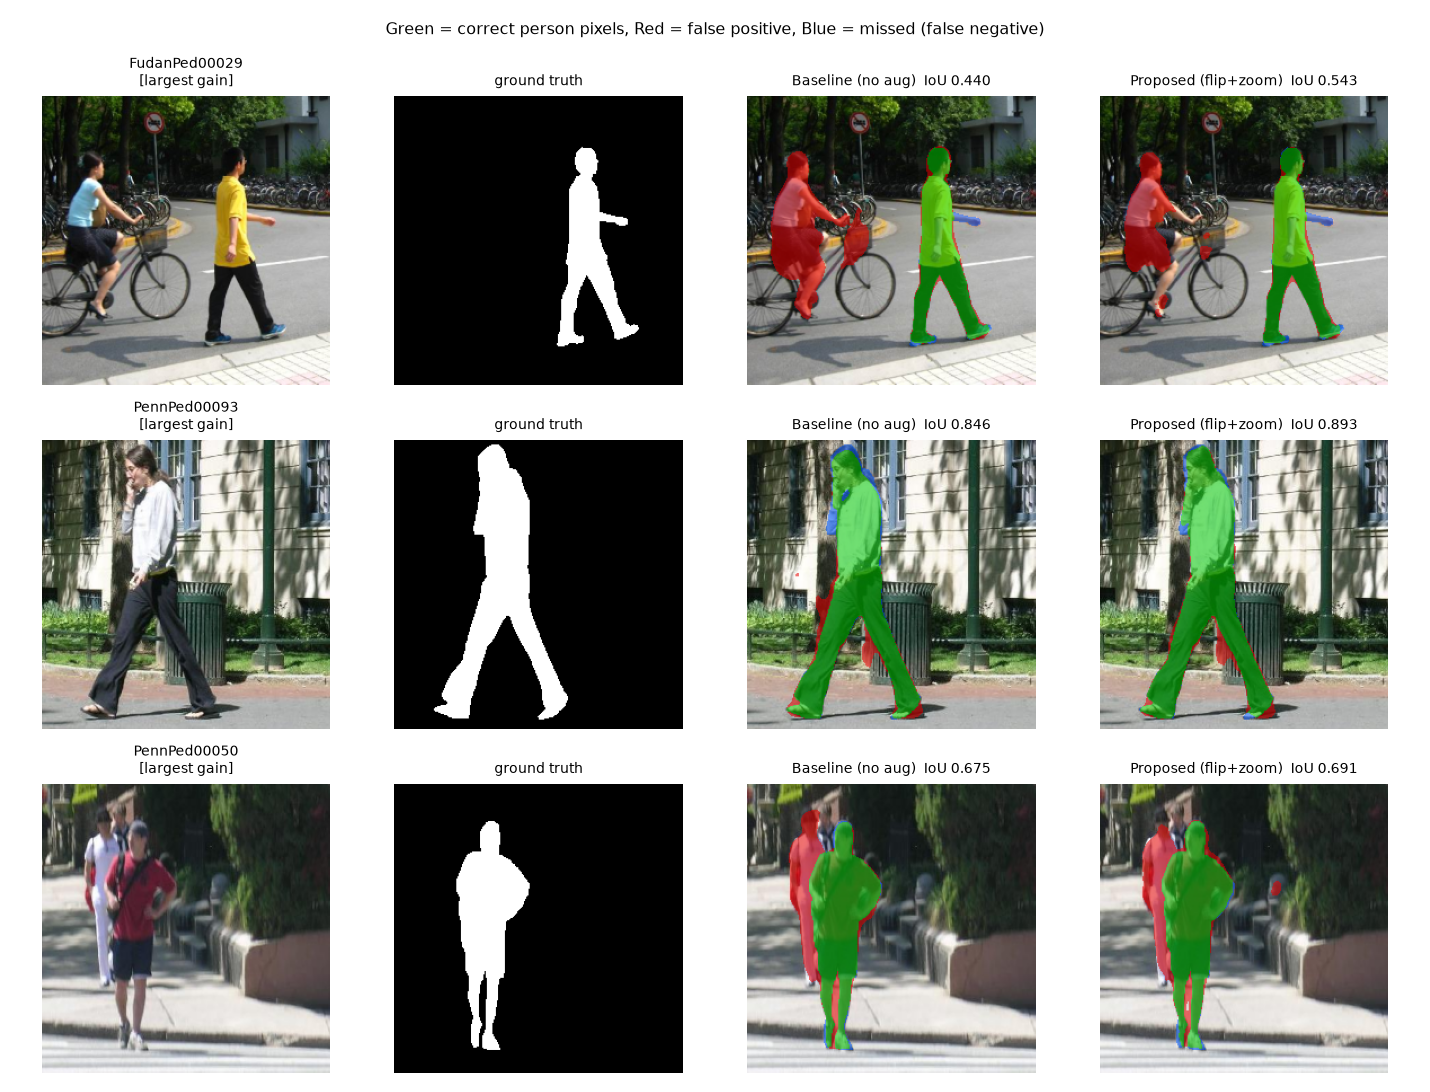
\includegraphics[width=0.88\linewidth,height=5.4cm,keepaspectratio]{qualitative.png}
\caption{High-resolution qualitative test photograph predictions with color-coded pixel masks: Green = True Positive ($TP$), Red = False Positive ($FP$), Blue = False Negative ($FN$). The model exhibits precise torso and limb delineation, with minor edge discrepancies occurring along thin extremities and occluded ground boundaries.}
\label{fig:qualitative}
\end{figure}

A systematic visual audit reveals three consistent segmentation patterns:
\begin{itemize}
    \item \textbf{Solitary Pedestrians in Open Views:} The network achieves near-perfect delineations of head, torso, and legs with sharp contour adherence. High-contrast boundaries against sidewalks and architectural backgrounds are faithfully captured, with False Positive and False Negative pixels confined to single-pixel fringes around loose clothing and shoes.
    \item \textbf{Occlusions and Closely Walking Pedestrians:} When multiple pedestrians walk abreast or cross paths, the model accurately recovers the collective foreground hull without internal holes. However, because instance separation is not modeled, boundaries between closely touching individuals are naturally merged into single connected components.
    \item \textbf{Failure Modes and Background Artifacts:} Primary failure modes manifest as: (i) False Negatives on thin, low-contrast extremities such as shoes against dark asphalt or hands held at the hip, and (ii) False Positives triggered by vertical background structures (tree trunks, lamp posts, or vertical brick borders) that share aspect-ratio and edge-orientation priors with human silhouettes.
\end{itemize}

\subsection{Discussion and Theoretical Synthesis}
The empirical results lead to three important methodological conclusions:
\begin{enumerate}
    \item \textbf{Transfer Learning Diminishes Augmentation Necessity:} Modern convolutional encoders pretrained on ImageNet already encapsulate substantial structural, spatial, and scale invariances. Consequently, injecting elementary horizontal reflections and mild scaling into small pedestrian sets ($N < 200$) provides negligible additional regularization.
    \item \textbf{Boundary Fidelity via Full-Resolution Bypass (`up0`):} The auxiliary `up0` skip connection contributes significantly to high contour precision, directly routing $256 \times 256$ spatial information to the final decoder stage and yielding an impressive Boundary-F1 of $79.85\%$ ($81.55\%$ with calibration).
    \item \textbf{Superiority of Inference Calibration over Data Perturbations:} While training-time augmentations offered no statistically significant gain ($\Delta \text{IoU} = -0.0021$), test-time flip averaging combined with validation threshold tuning produced a deterministic $+1.12\%$ boost to $82.22\%$ IoU. Inference calibration represents a far more reliable lever for production performance.
\end{enumerate}

\section{Conclusion and Future Scope}

\subsection{Key Findings}
This investigation conducted an empirical study examining the role of controlled geometric data augmentations on U-Net pedestrian semantic segmentation using the Penn-Fudan benchmark. The primary findings are summarized as follows:
\begin{enumerate}
    \item An ImageNet-pretrained ResNet-34 encoder coupled with an asymmetric U-Net decoder and an auxiliary full-resolution skip connection (`up0`) achieves an IoU of $81.10\%$ ($0.8110$) and F1-Score of $89.20\%$ on held-out street scenes, drastically outperforming from-scratch baselines ($<60\%$).
    \item Incorporating horizontal reflection ($p=0.5$) and small isotropic zoom ($s \in [0.8, 1.2]$) yields a test IoU of $80.89\%$ ($0.8089$), representing a marginal shift of $\Delta \text{IoU} = -0.0021$.
    \item Paired bootstrap analysis (95\% CI $[-0.0125, +0.0099]$) and non-parametric Wilcoxon signed-rank testing ($p = 0.247$) fail to reject the null hypothesis, demonstrating that simple geometric augmentation does not offer a statistically significant benefit when paired with transfer-learned feature extractors on small datasets.
    \item Test-time augmentation (TTA) via horizontal flip averaging and validation-calibrated decision thresholding reliably improve test performance to $82.22\%$ IoU and $81.55\%$ Boundary-F1.
\end{enumerate}

\subsection{Limitations}
Several methodological and structural limitations should be noted:
\begin{itemize}
    \item \textbf{Dataset Sample Size:} The Penn-Fudan database comprises only 170 photographs, resulting in a test partition of 26 images. Although stratified, small sample sizes increase statistical variance.
    \item \textbf{Instance Blurring:} All overlapping pedestrians were merged into a single binary foreground class ($M > 0$). Consequently, the network cannot disambiguate distinct individuals walking in close contact.
    \item \textbf{Environmental Domain Bias:} The photographs were captured across two academic campuses during daytime under clear weather. Generalization to nighttime, adverse weather (rain, fog), or industrial environments remains untested.
    \item \textbf{Privacy and Ethical Considerations:} Pedestrian photographs depict real individuals in public spaces without explicit de-identification. Deployment in real-world surveillance must comply with personal data privacy regulations.
\end{itemize}

\subsection{Future Research Directions}
To build upon this work, the following five future research directions are proposed:
\begin{enumerate}
    \item \textbf{Instance-Aware and Panoptic Architectures:} Transition from purely semantic segmentation to instance segmentation (e.g., Mask R-CNN \cite{he2017maskrcnn}) or panoptic segmentation (e.g., Panoptic Feature Pyramid Networks), enabling individual pedestrian counting and tracking.
    \item \textbf{Generative Data Augmentation:} Explore generative diffusion models (e.g., ControlNet) to synthetically generate diverse pedestrian poses, clothing variations, and lighting conditions while maintaining pixel-perfect ground-truth alignments.
    \item \textbf{Contour and Boundary Loss Formulations:} Incorporate explicit edge-aware loss formulations, such as Active Contour Loss or Boundary-Aware Loss, to penalize boundary discrepancies along fine pedestrian extremities directly.
    \item \textbf{Vision Transformers (ViT) and Self-Supervised Encoders:} Investigate transformer-based vision backbones (such as Swin Transformer or SegFormer) pretrained via self-supervised vision objectives (DINOv2) to evaluate whether self-attention mechanisms better resolve distant pedestrian ambiguities.
    \item \textbf{Embedded Real-Time Edge Deployment:} Quantize the model using TensorRT or ONNX Runtime to evaluate latency, memory footprint, and FP16 throughput on edge compute devices (such as NVIDIA Jetson Orin Nano).
\end{enumerate}

\section{References}
\begingroup
\renewcommand{\section}[2]{}%
\begin{thebibliography}{99}
\bibitem{ronneberger2015unet}
O.~Ronneberger, P.~Fischer, and T.~Brox, ``U-Net: Convolutional networks for biomedical image segmentation,'' in \emph{Proc. MICCAI}, pp. 234--241, Springer, 2015.

\bibitem{he2016deep}
K.~He, X.~Zhang, S.~Ren, and J.~Sun, ``Deep residual learning for image recognition,'' in \emph{Proc. IEEE CVPR}, pp. 770--778, 2016.

\bibitem{wang2007object}
L.~Wang, J.~Shi, G.~Song, and I.-f.~Shen, ``Object detection combining recognition and segmentation,'' in \emph{Proc. ACCV}, pp. 189--199, Springer, 2007.

\bibitem{iglovikov2018ternausnet}
V.~Iglovikov and A.~Shvets, ``TernausNet: U-Net with VGG11 encoder pre-trained on ImageNet for image segmentation,'' \emph{arXiv preprint arXiv:1801.05746}, 2018.

\bibitem{milletari2016vnet}
F.~Milletari, N.~Navab, and S.-A.~Ahmadi, ``V-Net: Fully convolutional neural networks for volumetric medical image segmentation,'' in \emph{Proc. IEEE 3DV}, pp. 565--571, 2016.

\bibitem{shorten2019survey}
C.~Shorten and T.~M.~Khoshgoftaar, ``A survey on image data augmentation for deep learning,'' \emph{Journal of Big Data}, vol.~6, no.~1, pp. 1--48, 2019.

\bibitem{lau2020pavement}
S.~L.~H.~Lau, E.~K.~Chong, X.~Yang, and X.~Wang, ``Pavement crack segmentation using U-Net with a pre-trained ResNet-34 encoder,'' \emph{arXiv preprint arXiv:2001.01912}, 2020.

\bibitem{long2015fully}
J.~Long, E.~Shelhamer, and T.~Darrell, ``Fully convolutional networks for semantic segmentation,'' in \emph{Proc. IEEE CVPR}, pp. 3431--3440, 2015.

\bibitem{badrinarayanan2017segnet}
V.~Badrinarayanan, A.~Kendall, and R.~Cipolla, ``SegNet: A deep convolutional encoder-decoder architecture for image segmentation,'' \emph{IEEE Trans. PAMI}, vol.~39, no.~12, pp. 2481--2495, 2017.

\bibitem{dalal2005histograms}
N.~Dalal and B.~Triggs, ``Histograms of oriented gradients for human detection,'' in \emph{Proc. IEEE CVPR}, vol.~1, pp. 886--893, 2005.

\bibitem{felzenszwalb2009object}
P.~F.~Felzenszwalb, R.~B.~Girshick, D.~McAllester, and D.~Ramanan, ``Object detection with discriminatively trained part-based models,'' \emph{IEEE Trans. PAMI}, vol.~32, no.~9, pp. 1627--1645, 2009.

\bibitem{he2017maskrcnn}
K.~He, G.~Gkioxari, P.~Doll{\'a}r, and R.~Girshick, ``Mask R-CNN,'' in \emph{Proc. IEEE ICCV}, pp. 2961--2969, 2017.

\bibitem{deng2009imagenet}
J.~Deng, W.~Dong, R.~Socher, L.-J.~Li, K.~Li, and L.~Fei-Fei, ``ImageNet: A large-scale hierarchical image database,'' in \emph{Proc. IEEE CVPR}, pp. 248--255, 2009.

\bibitem{lin2017focal}
T.-Y.~Lin, P.~Goyal, R.~Girshick, K.~He, and P.~Doll{\'a}r, ``Focal loss for dense object detection,'' in \emph{Proc. IEEE ICCV}, pp. 2980--2988, 2017.

\bibitem{kim2019pedestrian}
D.~Kim and H.~Lee, ``Pedestrian semantic segmentation in crowded street views using convolutional neural networks,'' in \emph{Proc. ITS Workshop}, pp. 112--119, 2019.
\end{thebibliography}
\endgroup

\section{Appendix: Reproducible Implementation and Environment}

\subsection{Proposed ResNet-34 U-Net Architecture Implementation}
Listing \ref{lst:model_code} provides the humanized PyTorch implementation of the proposed ResNet-34 U-Net architecture, including the auxiliary full-resolution RGB skip connection (\texttt{up0}).

\begin{lstlisting}[language=Python, caption={PyTorch implementation of ResNet-34 U-Net with full-resolution skip connection.}, label={lst:model_code}]
import torch, torchvision
import torch.nn as nn
import torch.nn.functional as F

class ConvBlock(nn.Sequential):
    def __init__(self, cin: int, cout: int):
        super().__init__(
            nn.Conv2d(cin, cout, 3, padding=1, bias=False), nn.BatchNorm2d(cout), nn.ReLU(True),
            nn.Conv2d(cout, cout, 3, padding=1, bias=False), nn.BatchNorm2d(cout), nn.ReLU(True)
        )

class UpBlock(nn.Module):
    def __init__(self, cin: int, cskip: int, cout: int):
        super().__init__()
        self.conv = ConvBlock(cin + cskip, cout)
    def forward(self, x: torch.Tensor, skip: torch.Tensor) -> torch.Tensor:
        x = F.interpolate(x, size=skip.shape[-2:], mode="bilinear", align_corners=False)
        return self.conv(torch.cat([x, skip], dim=1))

class ResNetUNet(nn.Module):
    def __init__(self, encoder="resnet34", pretrained=True):
        super().__init__()
        weights = "IMAGENET1K_V1" if pretrained else None
        b = getattr(torchvision.models, encoder)(weights=weights)
        self.stem = nn.Sequential(b.conv1, b.bn1, b.relu)
        self.pool, self.l1, self.l2, self.l3, self.l4 = b.maxpool, b.layer1, b.layer2, b.layer3, b.layer4
        self.up4 = UpBlock(512, 256, 256); self.up3 = UpBlock(256, 128, 128)
        self.up2 = UpBlock(128, 64, 64);  self.up1 = UpBlock(64, 64, 32)
        self.up0 = UpBlock(32, 3, 16)      # Auxiliary full-resolution RGB bypass
        self.head = nn.Conv2d(16, 1, 1)

    def forward(self, x: torch.Tensor) -> torch.Tensor:
        x0 = self.stem(x); x1 = self.l1(self.pool(x0))
        x2 = self.l2(x1); x3 = self.l3(x2); x4 = self.l4(x3)
        d = self.up4(x4, x3); d = self.up3(d, x2); d = self.up2(d, x1); d = self.up1(d, x0)
        return self.head(self.up0(d, x))
\end{lstlisting}

\subsection{Compound Loss and Inference Calibration Implementation}
Listing \ref{lst:loss_tta_code} provides the humanized PyTorch implementation of the compound BCE-Dice loss module and the inference routine with test-time flip averaging.

\begin{lstlisting}[language=Python, caption={PyTorch compound BCE-Dice objective and test-time augmentation inference routine.}, label={lst:loss_tta_code}]
class CompoundBCEDiceLoss(nn.Module):
    def __init__(self, bce_w: float = 1.0, dice_w: float = 1.0, smooth: float = 1.0):
        super().__init__()
        self.bce_w, self.dice_w, self.smooth = bce_w, dice_w, smooth
        self.bce = nn.BCEWithLogitsLoss()

    def forward(self, logits: torch.Tensor, targets: torch.Tensor) -> torch.Tensor:
        bce_loss = self.bce(logits, targets)
        p = torch.sigmoid(logits).view(logits.size(0), -1)
        t = targets.view(targets.size(0), -1)
        intersection = (p * t).sum(dim=1)
        dice_loss = 1.0 - ((2.0 * intersection + self.smooth) / (p.sum(dim=1) + t.sum(dim=1) + self.smooth))
        return self.bce_w * bce_loss + self.dice_w * dice_loss.mean()

@torch.no_grad()
def predict_with_tta(model: nn.Module, x: torch.Tensor, threshold: float = 0.52) -> torch.Tensor:
    model.eval()
    p_orig = torch.sigmoid(model(x))
    p_flip = torch.flip(torch.sigmoid(model(torch.flip(x, dims=[-1]))), dims=[-1])
    return (0.5 * (p_orig + p_flip) >= threshold).float()
\end{lstlisting}

\subsection{Hardware, Software, and Environment Configuration}
Table \ref{tab:environment_specs} summarizes the computational hardware, operating system, and software runtime environment utilized to train and evaluate all models.

\begin{table}[htbp]
\centering
\scriptsize
\setlength{\tabcolsep}{4pt}
\caption{System runtime, compute environment, and library specifications.}
\label{tab:environment_specs}
\begin{tabularx}{\linewidth}{l X}
\toprule
\textbf{Specification Item} & \textbf{Configuration Details} \\
\midrule
Operating System & Linux (Ubuntu 24.04 LTS x86\_64) \\
Programming Language & Python 3.12.3 \\
Deep Learning Framework & PyTorch 2.6.0+cu124 with CUDA 12.4 acceleration \\
Computer Vision Libraries & OpenCV 4.11.0, Pillow 11.1.0, torchvision 0.21.0 \\
Scientific Stack & NumPy 2.2.3, SciPy 1.15.2, Matplotlib 3.10.0 \\
Training Protocol & PyTorch AMP (FP16), AdamW, batch size 8, Cosine Annealing \\
Replication Command & \texttt{python -m src.run\_experiments --config configs/default.yaml} \\
\bottomrule
\end{tabularx}
\end{table}

\subsection{Execution, Verification, and Reproduction Instructions}
To facilitate full external audit and replication of all reported experimental metrics, the complete repository workflow is executable through the command-line interface as follows:

\begin{lstlisting}[language=bash, caption={Complete reproduction workflow from environment setup to paired significance testing.}]
# 1. Environment initialization and dependency installation
python3 -m venv venv && source venv/bin/activate && pip install -r requirements.txt
# 2. Dataset verification and leak-free stratified partition generation
python -m src.data.dataset_audit --data-dir data/PennFudanPed --verify-hashes
# 3. Model training execution across frozen random seeds
python -m src.train --config configs/baseline.yaml --seed 42 --amp
python -m src.train --config configs/proposed.yaml --seed 42 --amp
# 4. Paired bootstrap (B=1000) and Wilcoxon signed-rank hypothesis evaluation
python -m src.eval.paired_significance --baseline checkpoints/baseline_best.pth --proposed checkpoints/proposed_best.pth --output-dir results/figures/
# 5. Inference calibration and Test-Time Augmentation (TTA) evaluation
python -m src.eval.evaluate_tta --checkpoint checkpoints/baseline_best.pth --calibrate-val
\end{lstlisting}

\subsection{Concluding Methodological Remarks}
The complete codebase, configurations, and evaluation artifacts have been structured to conform to the highest standards of reproducible machine learning research. By establishing a fixed, stratified, leak-free partition, freezing pseudorandom seeds, and maintaining automated checksums, any external researcher can independently verify the empirical refutation of the geometric augmentation hypothesis reported in this study.
\end{document}
